%!TEX root = ../report.tex
\section{Stream tubes}
\label{sec:stream_tubes}
In order to visualize stream tubes, a history of previous time frames is needed to show a trail of particles.

\subsection{History of time frames}
The model of the program did not store any data of previous time frames, so the model had to be changed. 
During every simulation step, the \texttt{solve} function calculates the vector field defined by \texttt{vx} and \texttt{vy}, which are the \(x\) and \(y\) components of the velocity vector field.
To keep track of the history of these values, a queue was created that stores pairs of pointers.
The first pointer of this pair is a pointer to the \(x\) components of the vector field, and the second pointer is a pointer to the \(y\) component of the vector field.
Since the queue keeps track of references instead of values, a copy of the current values has to be created and this copy needs to be stored.

The queue was designed to be a circular queue of size 100, this means that the data is pushed to the queue while the size is less than 100.
As soon as the size of the queue becomes 100, an element is popped first before the new value is pushed.
This mechanism makes sure that the size of the queue never becomes larger than 100. 
The benefit of using a circular queue is that the 100 most recent time frames are now stored, while not leaking memory by storing all time frames.

\subsection{Constructing stream tubes}
The trajectory of the stream tube traces out the path of a particle released at a placed seed, which is placed somewhere in the history of time frames.
The step in space that the stream tube takes at a time frame is determined by the value of the vector field at that time frame.
Let's say we have placed a seed at position \(\vec{p}_0 = \left(x_0, y_0\right)\), \(T_{back}\) timesteps back in history.
To determine the position \(\vec{p}_1\), which is \(T_{back} - 1\) timesteps back in history, we use the vector field that existed \(T_{back}\) timesteps ago:

\[
	\vec{p}_i = 
	\vec{p}_{i-1} + \Delta t \cdot \vec{v}_{i-1}\left( \vec{p}_{i-1} \right)
\]

The subscript notations indicate how many timesteps back in history the value was. \(\Delta t\) denotes the time step.
Decomposing this in the \(x\) and \(y\) dimensions, this is equivalent to:

\begin{align*}
	x_i &= x_{i-1} + \Delta t \cdot v_{x, i-1}\left( \vec{p}_{i-1} \right) \\
	y_i &= y_{i-1} + \Delta t \cdot v_{y, i-1}\left( \vec{p}_{i-1} \right)
\end{align*}

Now, to draw the stream tubes, we only have to draw the center of the \(i\)-th element at position \(\vec{p}_i\).

To express the magnitude of the vector field on the stream tube, the radius of the stream tube will have a value that is proportional to the squared magnitude:
\[
	m_i = k\cdot(v_{x, i-1}(\vec{p}_{i-1})^2 + v_{y, i-1}(\vec{p}_{i-1})^2)\text{,}
\]
where \(k\) is some proportionality constant.
Furthermore, this value is clamped so it has a maximum value of 20.
The color of the stream tube element is also determined by the value \(m_i\).

The tubes are drawn by drawing multiple OpenGL cylinders, based on the positions \(p_i\) and magnitudes \(m_i\).

\subsection{Stream tube interaction}
The user can add a new seed point by clicking the \emph{Add seed point} button, and subsequently clicking the simulation screen.
The user can remove the last placed seed point by clicking the \emph{Remove seed point} button.

The \(z\) value of the seed point can be modified.
This value corresponds with how far back in time the seed point is placed.
It is limited between 0 and -100, because it doesn't make any sense to place seed points in the future (there is no data there), and we only store the last 100 frames, so we can't go back further than 100 steps.

The \emph{displacement factor} \(f_d\) is a factor that is used to fictitiously exaggerate the particle movement by multiplying the displacement by a factor \(f_d\):
\[
	\vec{p}_i = 
	\vec{p}_{i-1} + f_d \cdot \vec{v}_{i-1}\left( \vec{p}_{i-1} \right) \cdot \Delta t
\]
This is of course not realistic in any sense, but the particle traces are more pronounced this way, which is useful to give a sense how the vector field progressed in time.

\begin{figure}[htb]
  \centering
  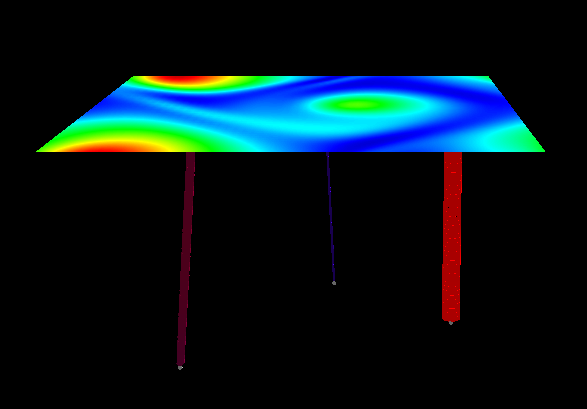
\includegraphics[width=\linewidth]{./content/pictures/stream_tubes.png}
  \caption{Three stream tubes. The seed points are drawn as gray spheres, and they are furthest back in time. The cylinders are shaded to give a clue on their perspective. The individual cylinders are almost indistinguishable, so it resembles a tube, but it isn't really.}
\end{figure}

\clearpage